\section{Background}

\subsection{Preliminaries\label{sec:pre}}
Given two graphs $q$ and $G$, the task of subgraph matching is to determine if the larger graph $G$ contains a subgraph that is isomorphic
to the query graph $q$. If the query and data graphs include vertex and edge labels, both the topology and the labels should be matched.
The large graph $G$ is known as a data or target graph.  Subgraph search is to find all subgraphs  of the data graph, which are isomorphic
to the query graph.

In this work, we target mining subgraphs from an \emph{undirected} and \emph{labeled} data graph $G=\{V,E,\Sigma,L_V,L_E\}$, where $V$, $E$
and $\Sigma$ are a set of vertices, edges and labels respectively,  $L_V$ is a function that associates a vertex $v \in V$ with a label
$L_V \in \Sigma$, and $L_E$ is a function that associates an edge $e \in E$ with a label $L_E \in \Sigma$. We describe a few important concepts of subgraph search as follows.

\cparagraph{Matching order.} Given a query graph $q$, a matching order $\pi$ is a permutation of vertices in $q$, where $\pi[i]$ is the
$i$th vertex in $\pi$. In essence, the matching order defines which order we match individual vertices of the query graph $q$ with the
counterparts from the data graph $G$. Studies have shown that choosing the right matching order can have a significant impact on
performance \cite{bi2016efficient,sun2020subgraph,sun2020rapidmatch,guo2020gpu}.  \SystemName provides a dedicated algorithm to generate
the matching order; see Section \ref {sec:matchingorder}.

\cparagraph{Embedding.} Given a query graph $q$ and a matching order $\pi$, \SystemName iteratively chooses  one or multiple unprocessed
vertices from the matching order $\pi$ to perform subgraph search. Before we match the last vertex in the matching order, we only apply a
sub-query graph. The subgraphs of $G$ that are isomorphic to the query graph or sub-query graph are called subgraph isomorphic embeddings.
A full subgraph isomorphic embedding is obtained if every vertex in the query graph $q$ is mapped to a vertex in the data graph $G$. For
example, for the query graph $q$ in Figure \FIXME{xxa} and the data graph $G$ in Figure \FIXME{xxb}, there are three subgraph isomorphic
embeddings of $q$ in $G$, which maps $(u1, u2, u3, u4, u5)$ to $(v0, v2, v1, v5, v4)$, $(v0, v2, v1, v5, v6)$ and $(v0, v2, v3, v5, v6)$,
respectively. For simplicity, we use the term ``\emph{embedding}"\footnote{Not to confuse with the term embeddings (e.g., a vector of
numerical values) used by deep neural networks.} to refer to ``subgraph isomorphic embedding" thereafter.

\cparagraph{Backward edge.} Given a query graph $q$ and a subgraph $q'$ of $q$, if an edge $e$ exists in $q$ but not in subgraph $q'$ and
$e$ connects two vertices of $q'$, we call $e$ the backward edge. \SystemName uses the backward edges to remove invalid graph embeddings,
e.g. subgraphs whose topology or vertex or edge labels do not match the query graph, $q$.  (see Section \ref{sec:eliphase}).

\begin{figure}[t!]
\centering
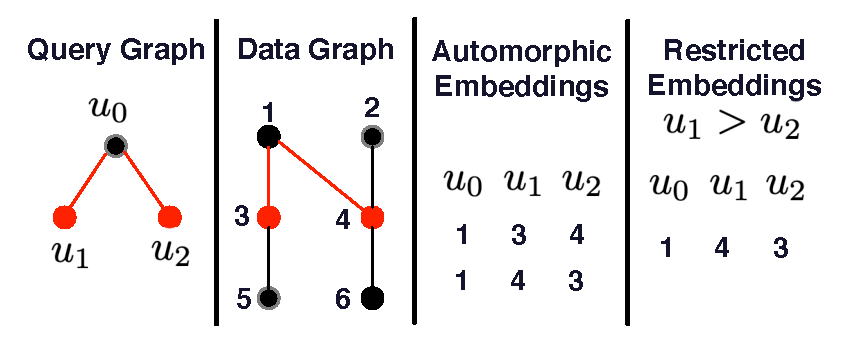
\includegraphics[width=\columnwidth]{./figure/automorphism.eps}
\caption{Examples of automorphic and non-automorphic embeddings.}	
\label{fig:automo}
\end{figure}

\cparagraph{Automorphism.} Given a graph $g$, an automorphism of $g$ is a match from $g$ to itself, which also indicates that $g$ is symmetric. Figure \ref{fig:automo} provides one of such examples, where the query graph has two symmetric vertices, $u_1$ and $u_2$, and two isomorphic embeddings (Figure \ref{fig:automo}c) that all corresponding to the same subgraph of the data graph with vertices $v_1, v_3, v_4$ (Figure \ref{fig:automo}b). To eliminate the duplicate embeddings, the standard practice is to impose some
restrictions on graph matching \cite{ mawhirter2019graphzero, shi2020graphpi}. Figure~\ref{fig:automo}d shows the matching criterion used
by GraphPi and GraphZero, which chooses an embedding where the data graph candidate vertex that has the largest number (i.e., we choose to
match $u_1$ with vertex $v_4$ rather than $v_3$ from the data graph) is chosen for a query graph vertex. This is a scheme used by GraphPi
\cite{shi2020graphpi} and GraphZero \cite{mawhirter2019graphzero}, and \SystemName also adopts this common practice.

\subsection{GPU Architecture\label{sec:gpu}}
GPUs are massively parallel computing devices. They are widely used to accelerate graph processing tasks, including subgraph matching
\cite{zeng2020gsi,guo2020exploiting,guo2020gpu}. GPU processing units can be abstracted into a two-level hierarchy, the Streaming
Multiprocessors (SMs) and computing cores inside the SM. An SM is further divided into processing blocks. Each processing block contains a
fixed number of threads, called a warp that is the basic scheduling unit.

Modern GPUs also organize their memory into a hierarchical system, containing the global memory, a configurable shared memory, registers,
and potentially an L2 cache between the global memory and the shared memory. The thread-local registers are the fastest memory component,
having the lowest access latency (1-2 cycles). The SM local L1 caches and shared memory provide a larger storage capacity over the
thread-local registers but have modestly higher accessing latency of around 30 cycles. Like the RAM in a CPU system, the GPU’s off-chip
global memory provides the largest memory storage capacity on the GPU but has the most expensive accessing latency of around 500 cycles.

The NVIDIA CUDA programming model provides atomic functions to perform a read-modify-write atomic operation on one 32-bit or 64-bit word
residing in global or shared memory. In this work, we use the CUDA $atomicAdd$ function. This function reads a variable in global memory
before adding a number to it and then writes the result back to the same address.
